\documentclass[10pt]{beamer}

\usepackage[utf8x]{inputenc}
\usepackage[OT4]{fontenc}

\usepackage[polish]{babel}

\setbeamertemplate{navigation symbols}{}

\usetheme[bullet=circle,
          titleline=true,
          pageofpages=z,
          alternativetitlepage=true]{Torino}

\usepackage{ragged2e}
\usepackage{hyphenat}
\usepackage{booktabs}
\usepackage{listings}
\usepackage{multibib}
\usepackage{multicol}
\usepackage[normalem]{ulem}

\usepackage{hyperref}
\hypersetup{colorlinks=true,urlcolor=blue}

\usepackage{tikz}
\usepackage{pgfplots}

\usetikzlibrary{arrows}
\usetikzlibrary{automata}
\usetikzlibrary{backgrounds}
\usetikzlibrary{decorations}

\usepackage{amsmath}
\usepackage{amsfonts}
\usepackage{amsthm}

\usepackage{pythonhighlight}

\title{SymPy --- czyli matematyka symboliczna w Pythonie}
\author{Mateusz Paprocki \texttt{<mattpap@gmail.com>}}
\institute{Continuum Analytics, Inc.}
\date{\today}

\setbeamercovered{transparent}

\begin{document}

\begin{frame}[plain,t]
    \maketitle
\end{frame}

\begin{frame}[fragile]
  \frametitle{Co to jest matematyka symboliczna?}
  \framesubtitle{}

  Python operuje na liczbach zmiennoprzecinkowych (IEEE-754):
  \begin{python}
    In[1]: import math
    In[2]: math.sqrt(3)
  \end{python}
  \begin{equation*}
    1.7320508075688772
  \end{equation*}

  W matematyce symbolicznej operujemy na liczbach i symbolach:
  \begin{python}
    In[3]: import sympy
    In[4]: sympy.sqrt(3)
  \end{python}
  \begin{equation*}
    \sqrt{3}
  \end{equation*}

  \begin{python}
    In[5]: _4.evalf()
  \end{python}
  \begin{equation*}
  1.73205080756888
  \end{equation*}

  \begin{python}
    In[6]: _4.evalf(n=50)
  \end{python}
  \begin{equation*}
    1.7320508075688772935274463415058723669428052538104
  \end{equation*}
\end{frame}

\begin{frame}[fragile]
  \frametitle{Co to jest matematyka symboliczna?}
  \framesubtitle{Dokładne wyniki}

  \begin{python}
    In[7]: math.sqrt(3)**2
  \end{python}
  \begin{equation*}
    2.9999999999999996
  \end{equation*}

  \begin{python}
    In[8]: sympy.sqrt(3)**2
  \end{python}
  \begin{equation*}
    3
  \end{equation*}

  \begin{python}
    In[9]: 1 - math.sin(math.pi)
  \end{python}
  \begin{equation*}
    0.9999999999999999
  \end{equation*}

  \begin{python}
    In[10]: 1 - sympy.sin(sympy.pi)
  \end{python}
  \begin{equation*}
    1
  \end{equation*}
\end{frame}

\begin{frame}[fragile]
  \frametitle{Co to jest matematyka symboliczna?}
  \framesubtitle{Operacje na symbolach i wyrażeniach}

  \begin{python}
  In[11]: x**2 - 1
  NameError: name 'x' is not defined
  \end{python}

  \begin{python}
  In[12]: f = lambda x: x**2 - 1
  In[13]: f(10)
  \end{python}
  \begin{equation*}
  99
  \end{equation*}

  \begin{python}
  In[14]: sympy.var('x')
  \end{python}
  \begin{equation*}
  x
  \end{equation*}

  \begin{python}
  In[15]: x**2 - 1
  \end{python}
  \begin{equation*}
  x^{2} - 1
  \end{equation*}

  \begin{python}
  In[16]: _.subs(x, 10)
  \end{python}
  \begin{equation*}
  99
  \end{equation*}

  \begin{python}
  In[17]: sympy.factor(_15)
  \end{python}
  \begin{equation*}
  \left(x - 1\right) \left(x + 1\right)
  \end{equation*}
\end{frame}

\begin{frame}[fragile]
  \frametitle{Co to jest matematyka symboliczna?}
  \framesubtitle{Wzory ogólne}

  \begin{python}
  In[18]: sum([ i for i in range(0, 10+1) ])
  \end{python}
  \begin{equation*}
  55
  \end{equation*}

  \begin{python}
  In[19]: n, k = sympy.symbols('n,k')
  In[20]: sympy.summation(k, (k, 0, n))
  \end{python}
  \begin{equation*}
  \frac{n^{2}}{2} + \frac{n}{2}
  \end{equation*}

  \begin{python}
  In[21]: _.subs(n, 10)
  \end{python}
  \begin{equation*}
  55
  \end{equation*}
\end{frame}

\begin{frame}[fragile]
  \frametitle{Matematyka w Pythonie}
  \framesubtitle{}

  \begin{itemize}
    \item moduł \texttt{math}
      \begin{itemize}
        \item wbudowany moduł matematyczny
        \item podstawowe operacje na liczbach zmiennoprzecinkowych
      \end{itemize}
    \item NumPy, SciPy
      \begin{itemize}
        \item biblioteki numeryczne (macierze, optymalizacja)
      \end{itemize}
    \item Swiginac, Pynac, \ldots
      \begin{itemize}
        \item warstwa abstrakcji nad biblioteką GiNaC (C++)
        \item duża wydajność, ale mała funkcjonalność
        \item trudne w rozwijaniu
      \end{itemize}
    \item Sage
      \begin{itemize}
        \item kompletny system algebry komputerowej
        \item podstawowy instalator to 0.8-1.4 GB (Linux 64)
        \item zawiera SymPy
      \end{itemize}
    \item SymPy
  \end{itemize}
\end{frame}

\begin{frame}[fragile]
  \frametitle{Dlaczego SymPy?}

  Istnieje wiele systemów matematycznych:
  \begin{itemize}
    \item systemy \structure{komercyjne}:
      \begin{itemize}
        \item Mathematica, Maple, Magma, \ldots
      \end{itemize}
    \item systemy \structure{Open Source}:
      \begin{itemize}
        \item AXIOM, GiNaC, Maxima, PARI, Sage, Singular, Yacas, \ldots
      \end{itemize}
  \end{itemize}
  \pause
  {\color{red} Problemy:}
  \begin{itemize}
    \item większość wymyśla swój własny język programowania
    \item trudna lub niemożliwa rozbudowa systemu i naprawa błędów
    \item systemy komercyjne są bardzo kosztowne
  \end{itemize}
\end{frame}

\begin{frame}
  \frametitle{Co to jest SymPy?}
  \framesubtitle{}

  \begin{itemize}
    \item biblioteka pisana w Pythonie
      \begin{itemize}
        \item \texttt{import sympy} i możemy całkować
        \item bez nowego środowiska, języka, \ldots
        \item bez rozszerzeń kompilowanych
        \item brak obligatoryjnych zależności (poza mpmath)
        \item działa dowolnej platformie (\sout{Jython})
      \end{itemize}
    \item prostota architektury
      \begin{itemize}
        \item kod w bibliotece oraz REPL nie powinny się (bardzo) różnić
        \item łatwość w rozbudowie na dowolnym poziomie
      \end{itemize}
    \item szeroka funkcjonalność
      \begin{itemize}
        \item obsługa najważniejszych gałęzi matematyki
        \item wspieranie zaawansowanych metod i algorytmów
        \item integracja z IPython/Jupiter, NumPy, \ldots
      \end{itemize}
    \item liberalna licencja: BSD
  \end{itemize}
\end{frame}

\begin{frame}[fragile]
  \frametitle{SymPy: historia i trochę liczb}

  \begin{itemize}
    \item 2006--teraz (Ondřej Čertík, od 2011 Aaron Meurer)
    \item 400 autorów
    \item 450+ tysięcy linii kodu, testów i dokumentacji
    \item wykonanie testów (na Travis CI) trwa średnio 9 godzin
    \item 48 projektów (45 studentów) w Google Summer of Code
  \end{itemize}
\end{frame}

\begin{frame}{Możliwości}
  \scriptsize
  \begin{multicols}{2}
    \begin{itemize}
      \item \textbf{podstawowe możlowści}
        \begin{itemize}
          \tiny
          \item podstawowa arytmetyka: +, -, *, /, **
          \item liczby dowolnej precyzji
          \item rozwijanie wyrażeń
          \item podstawianie wyrażeń
          \item upraszczanie/przekształcanie wyrażeń
          \item dopasowywanie do wzorców
          \item wyrażenia nieprzemienne
          \item stałe matematyczne ($\pi$, $e$, złoty podział)
        \end{itemize}
      \item \textbf{funkcje}
        \begin{itemize}
          \tiny
          \item elementarne (trygonometryczne, hiperboliczne, wykładnicza, logarytmy)
          \item kombinatoryczne, całkowitoliczbowe ($n!$, liczby Stirlinga)
          \item komponenty liczb zespolonych ($\Re{x}$, $\Im{x}$, $\left|{x}\right|$)
          \item wielomiany specjalne (cyklotomiczne, Czebyszewa)
          \item harmoniki sferyczne
          \item inne funkcje specjalne ($\Gamma{\left(x \right)}$, $\zeta{\left(x \right)}$)
        \end{itemize}
      \item \textbf{analiza matematyczna}
        \begin{itemize}
          \tiny
          \item różniczkowanie
          \item całkowanie
          \item granice
          \item szeregi (Taylor, Laurent, Puiseux)
        \end{itemize}
      \item \textbf{algebra wielomianów}
        \begin{itemize}
          \tiny
          \item artymetyka, największy wspólny dzielnik
          \item rozkład na czynniki
          \item rozkład bezkwadratowy
          \item bazy Gröbnera
          \item rozkład na ułamki proste
          \item wyróżnik i rugownik
          \item izolacja pierwiastków
        \end{itemize}
      \item \textbf{rozwiązywanie równań}
        \begin{itemize}
          \tiny
          \item równania wielomianowe
          \item równania algebraiczne
          \item równania transcendentalne
          \item równania różniczkowe
          \item równania różnicowe
          \item równania diofantyczne
          \item równania zadane przedziałami
          \item układy równań
          \item nierówności
        \end{itemize}
      \item \textbf{kombinatoryka}
        \begin{itemize}
          \tiny
          \item permutacje, kombinacje,partycje, podzbiory
          \item grupy permutacji (wielościany, kostka Rubkika)
          \item kody Prüfera, Graya
        \end{itemize}
    \end{itemize}
  \end{multicols}
\end{frame}

\begin{frame}{Więcej możliwości}
  \scriptsize
  \begin{multicols}{2}
    \begin{itemize}
      \item \textbf{matematyka dyskretna}
        \begin{itemize}
          \tiny
          \item współczynniki dwumianowe
          \item funkcje hipergeometryczne
          \item sumy i produkty (skończone i nieskończone)
      \end{itemize}
      \item \textbf{teoria liczb}
        \begin{itemize}
          \tiny
          \item generowanie i rozpoznawanie liczb pierwszych
          \item rozkład liczb całkowitych na czynniki
          \item ułamki łańcuchowe
        \end{itemize}
      \item \textbf{macierze}
        \begin{itemize}
          \tiny
          \item arytmetyka, odwracanie macierzy
          \item wartości i wektory własne
          \item wielomian charakterystyczny
          \item wyznacznik
        \end{itemize}
      \item \textbf{Geometry}
        \begin{itemize}
          \tiny
          \item punkty, linie, segmenty, elipsy, wielokąty, \ldots
          \item przecinanie się, styczność, podobieństwo figur
        \end{itemize}
      \item \textbf{fizyka}
        \begin{itemize}
          \tiny
          \item jednostki miar (analiza wymiarowa)
          \item stałe fizyczne
          \item mechanika klasyczne (dynamika bryły sztywnej)
          \item mechanika kwantowa (algebry Pauliego, algorytm Shora)
          \item optyka
        \end{itemize}
      \item \textbf{statystyka i rachunek prawdopodobieństwa}
        \begin{itemize}
          \tiny
          \item rozkłady prawdopodobieństwa
        \end{itemize}
      \item \textbf{wyświetlanie wyrażeń}
        \begin{itemize}
          \tiny
          \item 2D ASCII/Unicode
          \item LaTeX, MathML
          \item integracja z IPython/Jupyter notebook
          \item generacja kodu: C, Fortran, Python, JavaScript
        \end{itemize}
      \item \textbf{rysowanie wykresów}
        \begin{itemize}
          \tiny
          \item 2D i 3D
          \item krzywe parametryczne
          \item figury geometryczne
        \end{itemize}
    \end{itemize}
  \end{multicols}
\end{frame}

\begin{frame}[fragile]
  \frametitle{Przykłady}
  \framesubtitle{Podstawowa arytmetyka}

  SymPy automatycznie stosuje podstawowe transformacje:
  \begin{python}
    In[1]: 1 + x - y - y - x**2/x, exp(1), sin(0)
  \end{python}
  \begin{equation*}
    \left ( - 2 y + 1, \quad e, \quad 0\right )
  \end{equation*}
  Zaawansowane transformacje aplikowane są manualnie:
  \begin{python}
    In[2]: sin(x)**2 + cos(x)**2
  \end{python}
  \begin{equation*}
    \sin^{2}{\left (x \right )} + \cos^{2}{\left (x \right )}
  \end{equation*}

  \begin{python}
    In[3]: simplify(_)
  \end{python}
  \begin{equation*}
    1
  \end{equation*}
\end{frame}

\begin{frame}[fragile]
  \frametitle{Przykłady}
  \framesubtitle{Całkowanie i różniczkowanie}

  \begin{python}
    In[1]: integrate(sin(x*y*z), x, y)
  \end{python}
  \begin{equation*}
    \begin{cases} 0 & \text{for}\: y z = 0 \\- \frac{1}{z} \left(- \log{\left (x y z \right )} + \frac{1}{2} \log{\left (x^{2} y^{2} z^{2} \right )} + \operatorname{Ci}{\left (x y z \right )}\right) & \text{otherwise} \end{cases}
  \end{equation*}

  \begin{python}
    In[2]: diff(_, x, y)
  \end{python}
  \begin{equation*}
  \begin{cases} 0 & \text{for}\: y z = 0 \\\sin{\left (x y z \right )} & \text{otherwise} \end{cases}
  \end{equation*}

  \begin{python}
    In[3]: _1.subs({y: 0, z: 0})
  \end{python}
  \begin{equation*}
    0
  \end{equation*}

  \begin{python}
    In[4]: _1.args[1].expr.subs({y: 0, z: 0})
  \end{python}
  \begin{equation*}
    \mathrm{NaN}
  \end{equation*}
\end{frame}

\begin{frame}[fragile]
  \frametitle{Przykłady}
  \framesubtitle{Granice i szeregi}

  \begin{python}
    In[1]: lim = Limit((1 + 1/n)**n, n, oo)
    In[2]: Eq(lim, lim.doit())
  \end{python}
  \begin{equation*}
    \lim_{n \to \infty} \left(1 + \frac{1}{n}\right)^{n} = e
  \end{equation*}

  \begin{python}
    In[3]: limit(log(2 + sqrt(atan(x))*sqrt(sin(1/x))), x, 0)
  \end{python}
  \begin{equation*}
    \log{\left (2 \right )}
  \end{equation*}

  \begin{python}
    In[4]: series(sin(cos(x**2)), x, n=10)
  \end{python}
  \begin{equation*}
    \sin{\left (1 \right )} - \frac{x^{4}}{2} \cos{\left (1 \right )} + x^{8} \left(- \frac{1}{8} \sin{\left (1 \right )} + \frac{1}{24} \cos{\left (1 \right )}\right) + \mathcal{O}\left(x^{10}\right)
  \end{equation*}

  \begin{python}
    In[5]: summation(1/x**n, (n, 0, oo))
  \end{python}
  \begin{equation*}
    \begin{cases} \frac{1}{1 - \frac{1}{x}} & \text{for}\: \left|{\frac{1}{x}}\right| < 1 \\\sum_{n=0}^{\infty} x^{- n} & \text{otherwise} \end{cases}
  \end{equation*}
\end{frame}

\begin{frame}[fragile]
  \frametitle{Problemy i pułapki}
  \framesubtitle{liczby Pythona vs. liczby SymPy}

  \begin{python}
    In[1]: 1/2
  \end{python}
  \begin{equation*}
    0
  \end{equation*}

  \begin{python}
    In[2]: Rational(1, 2), S(1)/2, S("1/2"), S.Half
  \end{python}
  \begin{equation*}
    \left ( \frac{1}{2}, \quad \frac{1}{2}, \quad \frac{1}{2}, \quad \frac{1}{2}\right )
  \end{equation*}

  \pause

  \begin{python}
    In[3]: 1.23456789123456789
  \end{python}
  \begin{equation*}
    1.234567891234568
  \end{equation*}

  \begin{python}
    In[4]: Float(1.23456789123456789)
  \end{python}
  \begin{equation*}
    1.23456789123457
  \end{equation*}

  \begin{python}
    In[5]: Float("1.23456789123456789")
  \end{python}
  \begin{equation*}
    1.23456789123456789
  \end{equation*}
\end{frame}

\begin{frame}[fragile]
  \frametitle{Problemy i pułapki}
  \framesubtitle{porównywanie wyrażeń}

  \begin{python}
    In[1]: (x + 1)**2 == x**2 + 2*x + 1
  \end{python}
  \begin{equation*}
    \mathrm{False}
  \end{equation*}

  \begin{python}
    In[2]: (x + 1)**2 == (x + 1)**2
  \end{python}
  \begin{equation*}
    \mathrm{True}
  \end{equation*}

  \begin{python}
    In[3]: simplify((x + 1)**2 - x**2 + 2*x + 1) == 0
  \end{python}
  \begin{equation*}
    \mathrm{True}
  \end{equation*}

  \pause

  \begin{python}
    In[4]: Eq((x + 1)**2, x**2 + 2*x + 1)
  \end{python}
  \begin{equation*}
    \left(x + 1\right)^{2} = x^{2} + 2 x + 1
  \end{equation*}


\end{frame}

\begin{frame}[fragile]
  \frametitle{Problemy i pułapki}
  \framesubtitle{limit rekurencji i pamięć podręczna}

  \begin{python}
    In[1]: from sympy.core.cache import clear_cache
    In[2]: horner_poly = lambda n: horner(sum([ x**i for i in range(n) ]))
  \end{python}

  \begin{python}
    In[3]: clear_cache(); horner_poly(70).subs(x, 1)
    70
  \end{python}

  \begin{python}
    In[4]: clear_cache(); horner_poly(71).subs(x, 1)
    RuntimeError: maximum recursion depth exceeded
  \end{python}

  \pause

  \begin{python}
    In[5]: import sys
    In[6]: sys.setrecursionlimit(2*sys.getrecursionlimit())
  \end{python}

  \begin{python}
    In[7]: clear_cache(); horner_poly(142).subs(x, 1)
    142
  \end{python}

  \begin{python}
    In[8]: clear_cache(); horner_poly(143).subs(x, 1)
    RuntimeError: maximum recursion depth exceeded
  \end{python}
\end{frame}

\begin{frame}[fragile]
  \frametitle{Informacje kontaktowe}

  \begin{itemize}
    \item Strona główna projektu:
      \begin{itemize}
        \item \texttt{www.sympy.org}
      \end{itemize}
    \item Dokumentacja:
      \begin{itemize}
        \item \texttt{docs.sympy.org}
        \item \texttt{wiki.sympy.org}
      \end{itemize}
    \item Strony dodatkowe:
      \begin{itemize}
        \item \texttt{live.sympy.org}, \texttt{gamma.sympy.org}
        \item \texttt{try.jupyter.org}
      \end{itemize}
    \item Lista mailingowa:
      \begin{itemize}
        \item \texttt{sympy@googlegroups.com}
      \end{itemize}
    \item Kanał IRC:
      \begin{itemize}
        \item \texttt{\#sympy} na FreeNode
      \end{itemize}
    \item Repozytorium \texttt{git}:
    \begin{verbatim}
    git clone git://github.com/sympy/sympy.git
    \end{verbatim}
  \end{itemize}
\end{frame}

\begin{frame}[fragile]
  \frametitle{Dodatkowe materiały}

  \begin{itemize}
    \item \href{http://mattpap.github.com/scipy-2011-tutorial/html/index.html}{SymPy tutorial} at SciPy 2011
    \item \href{http://certik.github.io/scipy-2013-tutorial/html/index.html}{SymPy tutorial} at SciPy 2013 (\href{https://www.youtube.com/watch?v=dAgShwIx72c}{video})
    \item \href{https://github.com/pydy/pydy-tutorial-human-standing}{PyDy tutorial} at SciPy 2015 (\href{https://www.youtube.com/watch?v=mdo2NYtA-xY}{video})
  \end{itemize}
\end{frame}

\begin{frame}
  \frametitle{Moja rola w projekcie}
  \framesubtitle{}

  \begin{itemize}
    \item pracuję nad SymPy od marca 2007 roku
    \item student w Google Summer of Code 2007
      \begin{itemize}
        \item algorytmy rozwiązywania równań rekurencyjnych
        \item algorytmy sumowania nieoznaczonego i oznaczonego
      \end{itemize}
    \item no i tak już zostało:
      \begin{itemize}
        \item algorytmy całkowania
        \item wielomiany, struktury algebraiczne
        \item przekształcanie/upraszczanie wyrażeń
        \item \ldots
      \end{itemize}
    \item poza tym:
      \begin{itemize}
        \item mentor w Google Summer of Code 2009, 2010, 2011, 2013
        \item praca dyplomowa (Politechnika Wrocławska)
        \item konferencje (SciPy, EuroScipy, SciPy.In, PyCon.Pl, py4science)
      \end{itemize}
  \end{itemize}
\end{frame}

\begin{frame}
  \frametitle{Dziękuję za uwagę!}
  \framesubtitle{Pytania, uwagi, dyskusja \ldots}

  \vskip+1.0cm
  \begin{center}
    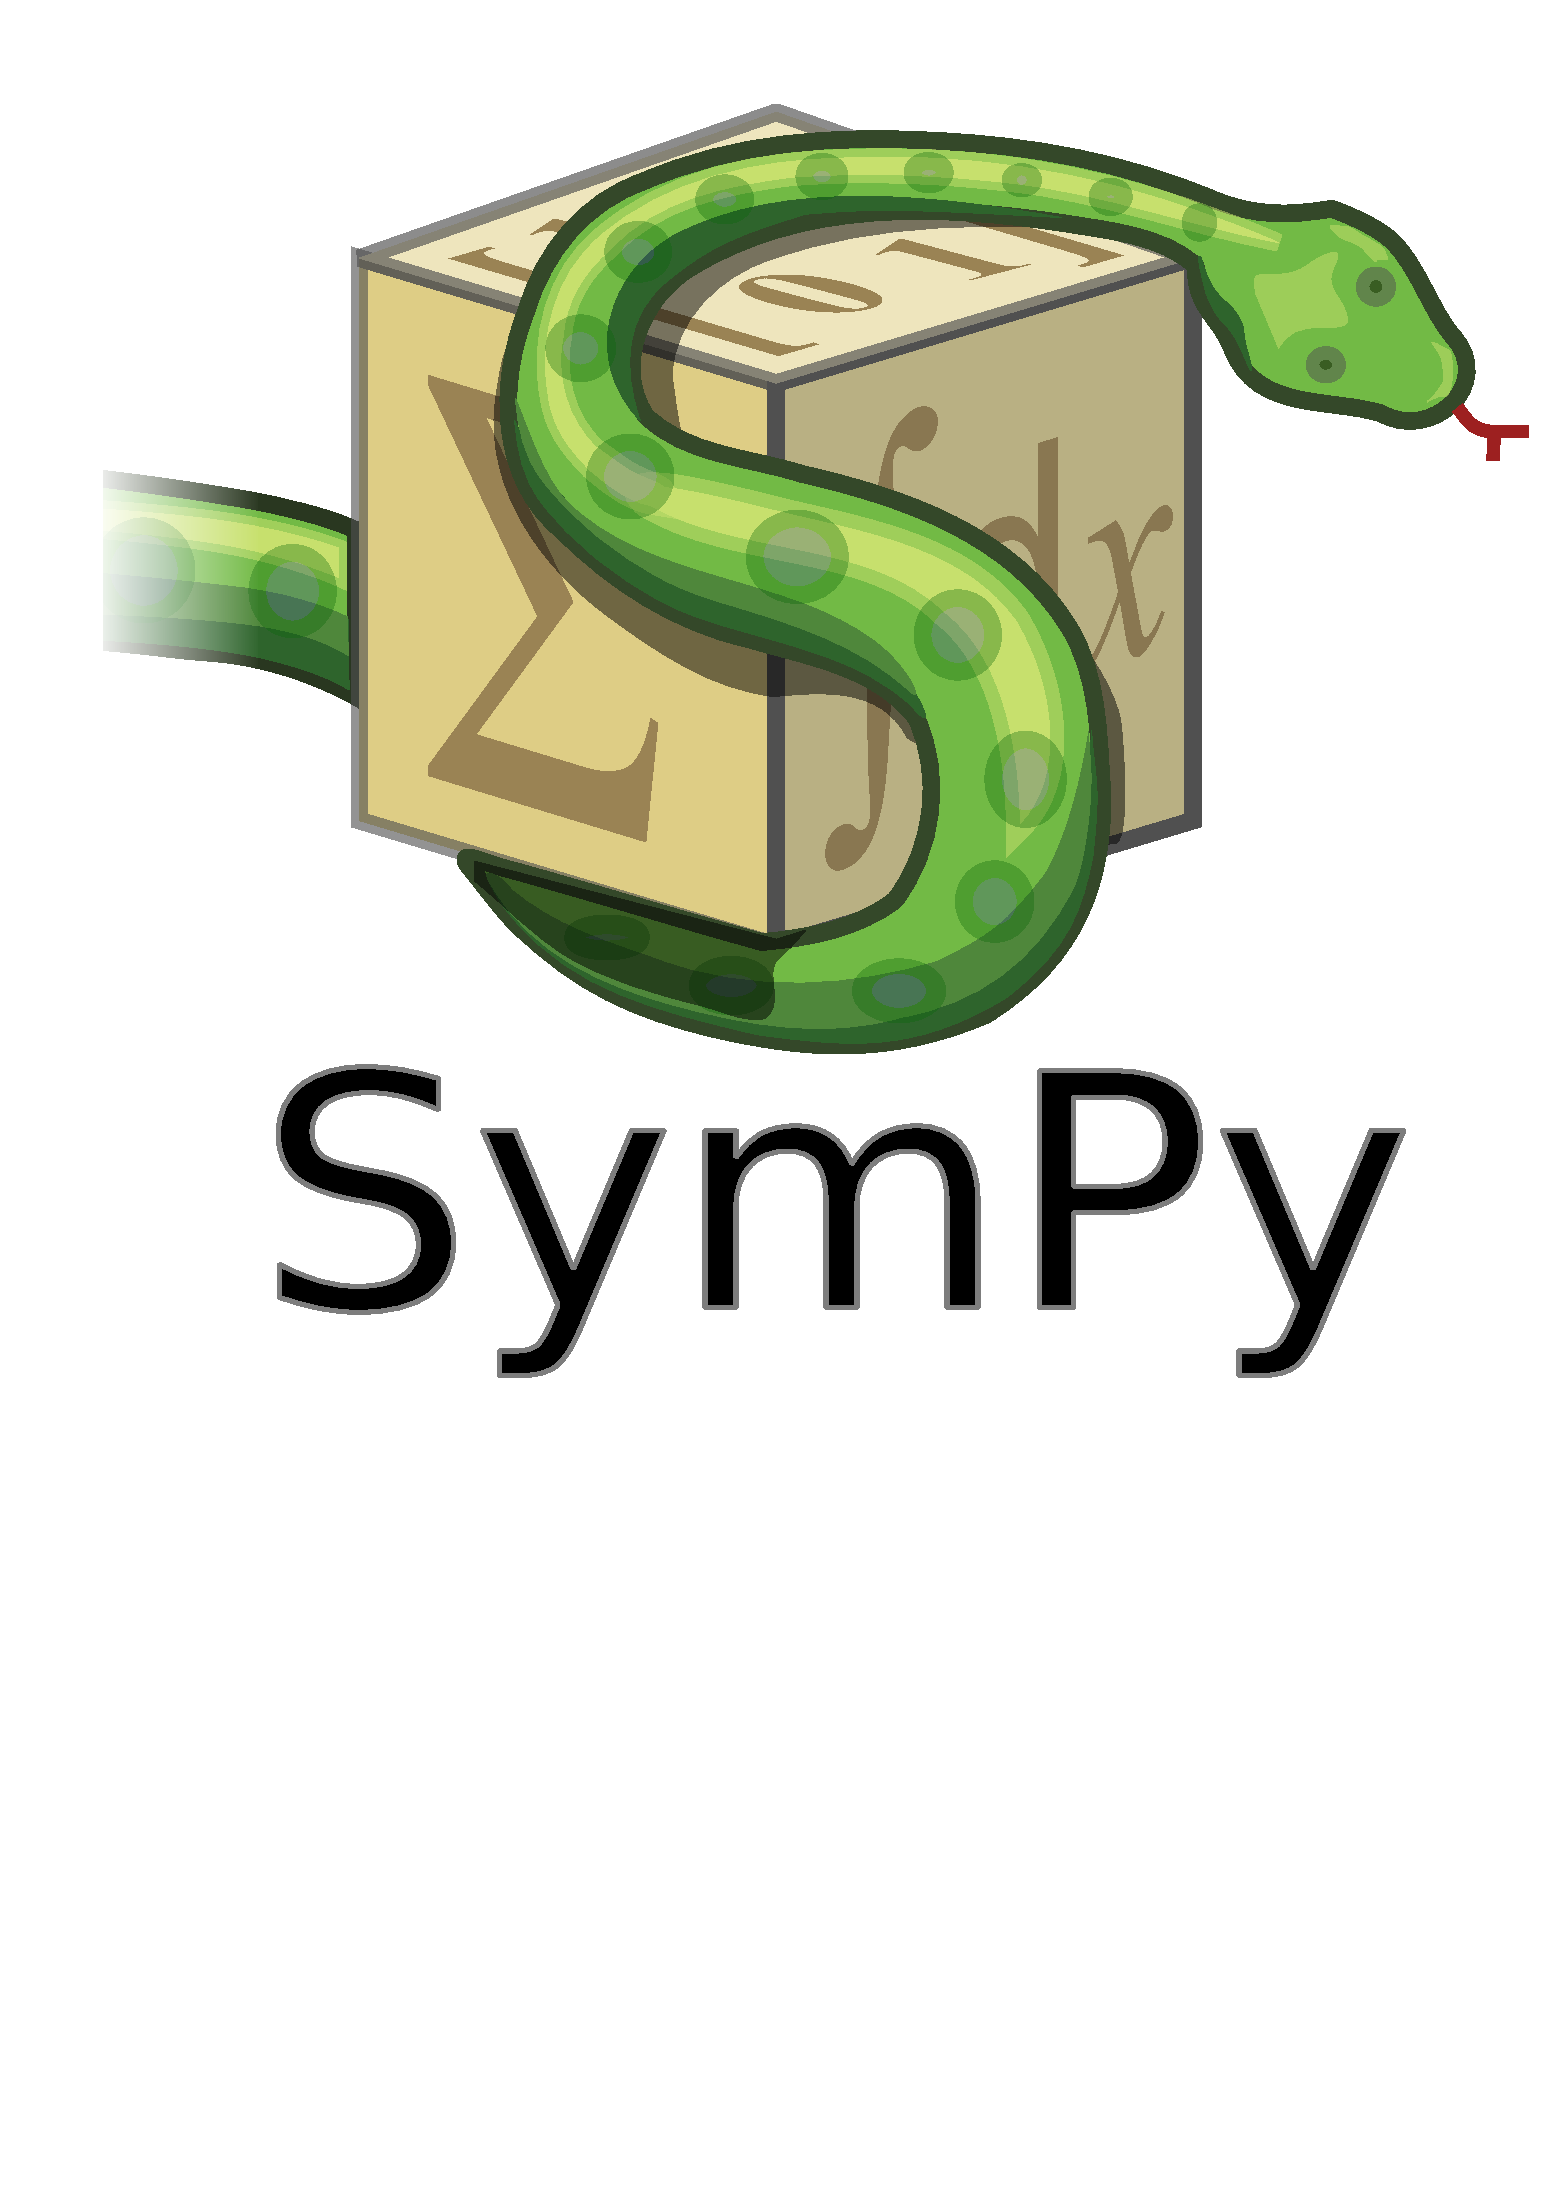
\includegraphics[scale=0.2]{images/sympy-logo.pdf}
  \end{center}
\end{frame}

\end{document}
